\documentclass[11pt]{article}
\usepackage{tikz}
\usetikzlibrary{intersections}
\usepackage{siunitx}
\usepackage{pgfplots}
\pgfplotsset{compat=1.15}

\begin{document}
	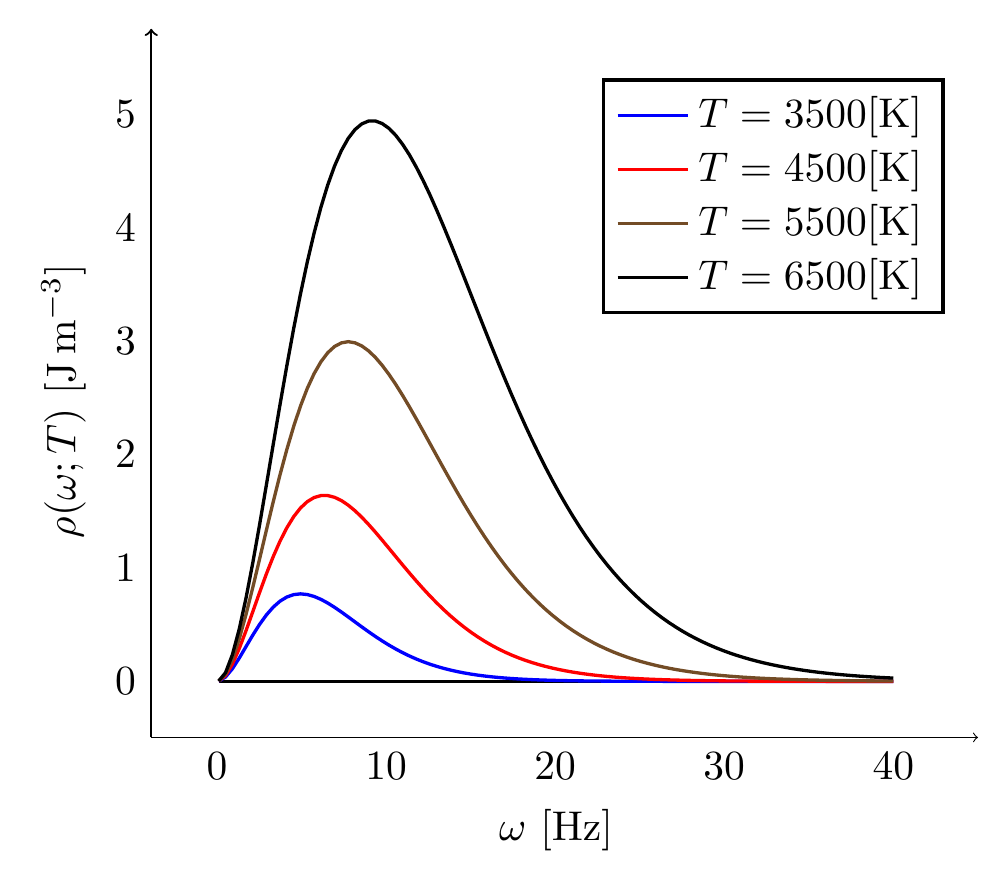
\begin{tikzpicture}[samples=100, scale=1.5]
		\draw[->,thick] {(0,0) -- (0,6)};
		\draw[->,thin] {(0,0) -- (7,0)};
    \begin{axis}[
        %xmin=0,
        xlabel={$\omega$ [\si{\hertz}]},
        %ymin=0,
        %ymax=pi,
        ylabel={$\rho (\omega; T)$ [\si{\joule\per\cubic\meter}]},
        %ytick=\empty,
        no markers,
        domain=0.1:40,
		  axis line style={draw=none},
		  tick style={draw=none},
        style={thick}]

       \addplot [forget plot,name path=B,samples=2] {0};

    \pgfplotsinvokeforeach{3500, 4500, 5500, 6500}
    {
        \addplot+ 
        {(x^3)/((pi^2)*(exp(2000*x/(#1))-1))};
        \addlegendentryexpanded{$T = #1 [\si{\kelvin}]$}
    }


    \end{axis}
    \end{tikzpicture}
    
\end{document}
